\documentclass[tikz,crop]{standalone}
\usetikzlibrary{angles,quotes,positioning,arrows,shapes,patterns,decorations,calc,decorations.pathreplacing,trees}
\usepackage[T1]{fontenc}
\usepackage{tgpagella} 
\usepackage{mathpazo}
\begin{document}
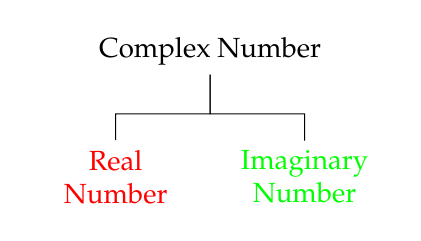
\begin{tikzpicture}[
        scale = 0.8,
        edge from parent fork down
    ]
    \node{Complex Number} [text width = 2cm,align = center,sibling distance = 3cm, level distance = 2cm]
    child{node[red] {Real Number}}
    child{node[green] {Imaginary Number}};
\end{tikzpicture}
\end{document}